\begin{figure}
	\centering
	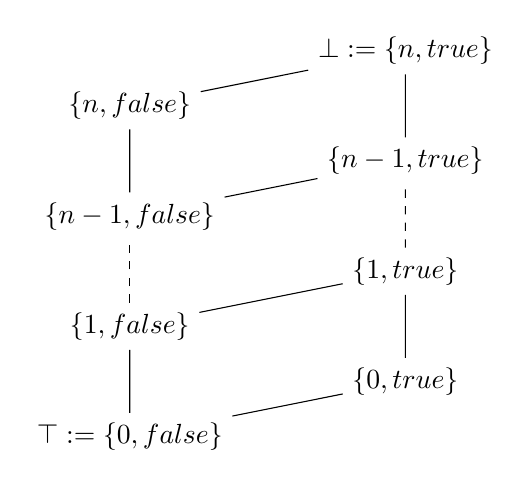
\begin{tikzpicture}[scale=.7]
		\node (np0) at(0,0) {$\top := \{0,false\}$};
		\node (np1) at(0,2) {$\{1,false\}$};
		\node (np2) at(0,4) {$\{n-1,false\}$};
		\node (np3) at(0,6) {$\{n,false\}$};
		\node (p0) at(5,1) {$\{0,true\}$};
		\node (p1) at(5,3) {$\{1,true\}$};
		\node (p2) at(5,5) {$\{n-1,true\}$};
		\node (p3) at(5,7) {$\bot := \{n,true\}$};
		\draw (np0) -- (p0) -- (p1) -- (np1) -- (np0);
		\draw (np2) -- (p2) -- (p3) -- (np3) -- (np2);
		\draw [dashed] (np1) -- (np2);
		\draw [dashed] (p1) -- (p2);
	\end{tikzpicture}
\caption{The definition of a upper bound compare node}
\label{fig:lattice}
\end{figure}